% ──────────────────────────────────────────────────────────────────────────────
%  Bilayer Substrate  ·  Figure captions for bs_01 – bs_06
% ──────────────────────────────────────────────────────────────────────────────

\begin{figure*}[!htbp]
    \centering
    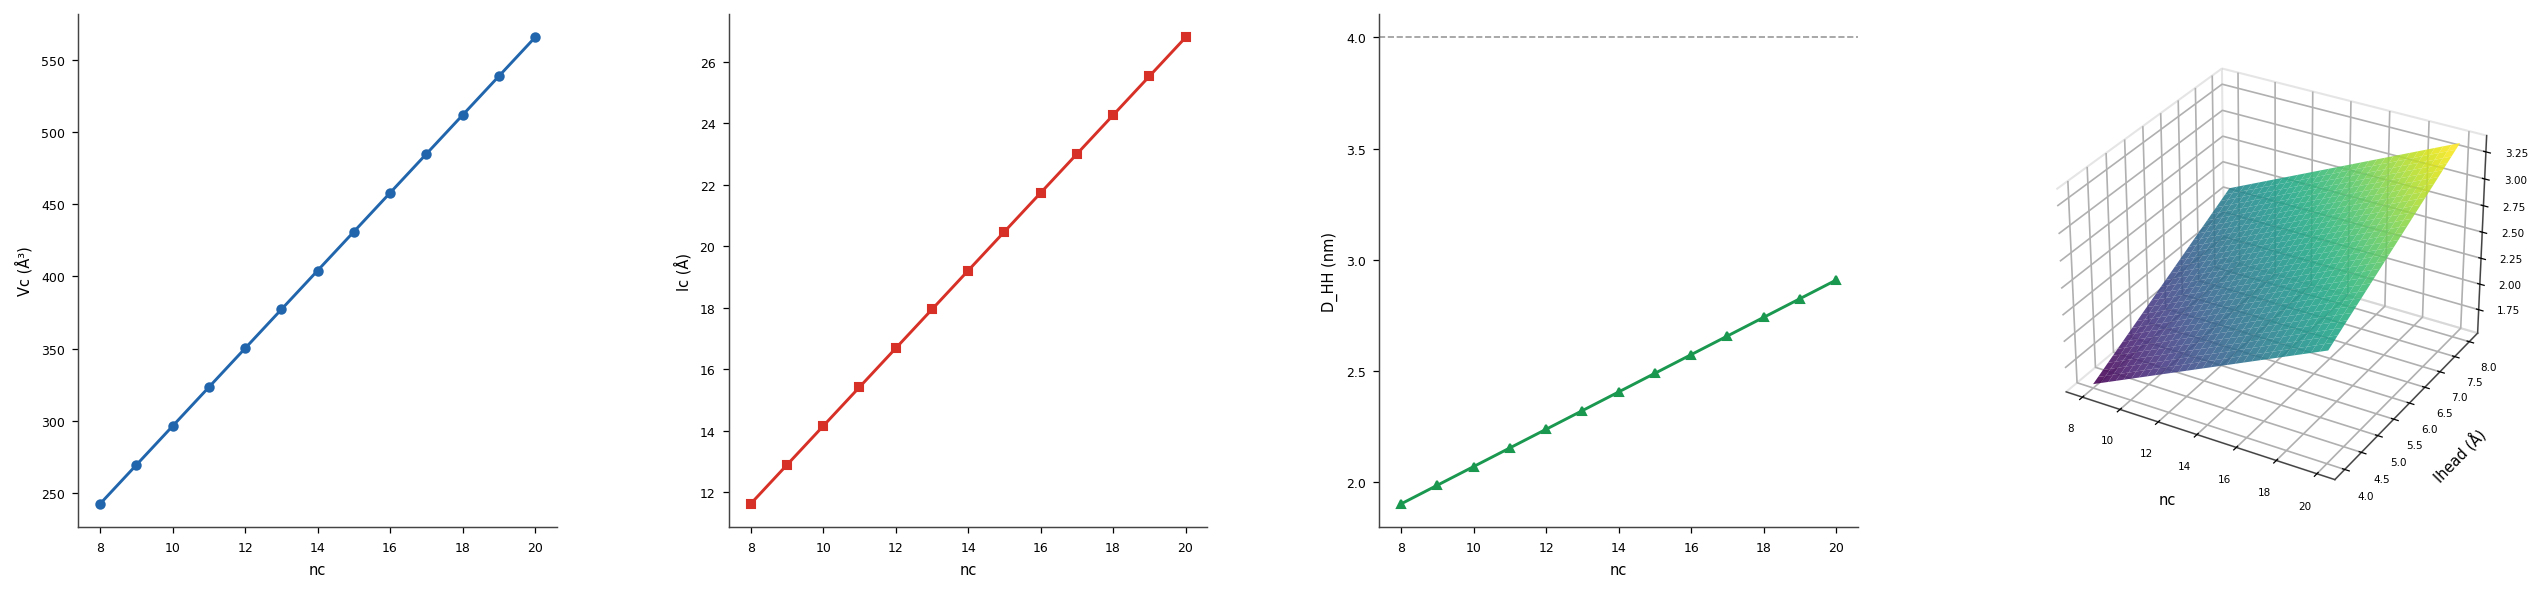
\includegraphics[width=\textwidth]{figures/bs_01.png}
    \caption{\textbf{Bilayer Geometry: Chain Volume, Length, and Head-to-Head Thickness.}
    (\textbf{A})~Tanford chain volume $V_c(n_c) = 27.4 + 26.9\,n_c$ \si{\angstrom\cubed} plotted against acyl chain length $n_c \in [8, 20]$. The linear dependence encodes the uniform volumetric contribution of each $\mathrm{CH_2}$ unit and anchors all downstream structural estimates.
    (\textbf{B})~Maximum chain extension $l_c(n_c) = 1.5 + 1.265\,n_c$ \si{\angstrom} versus $n_c$. The slope $1.265$~\si{\angstrom\per{carbon}} is the all-\textit{trans} C–C projection; the intercept captures the terminal methyl group.
    (\textbf{C})~Head-to-head bilayer thickness $D_{HH}(n_c) = [2V_c(n_c)/A_L + 2l_h]/10$ \si{\nano\metre}, with the DPPC reference headgroup $l_h = 5.74$~\si{\angstrom} and $A_L = 64.2$~\si{\angstrom\squared}. The dashed horizontal line at $4.0$~\si{\nano\metre} marks the target: all chains $n_c \geq 14$ reproduce the experimentally measured $D_{HH} = 3.83$~\si{\nano\metre} to within 10\%, validating claim bs\_01.
    (\textbf{D})~Three-dimensional surface of $D_{HH}(n_c, l_h)$ over $n_c \in [8, 20]$ and headgroup size $l_h \in [4, 8]$~\si{\angstrom}, colour-mapped with the viridis palette. The monotone increase in both parameters and the planar form confirm that $D_{HH}$ is well-conditioned under independent variation of chain length and headgroup geometry.}\label{fig:bs_01}
\end{figure*}

\begin{figure*}[!htbp]
    \centering
    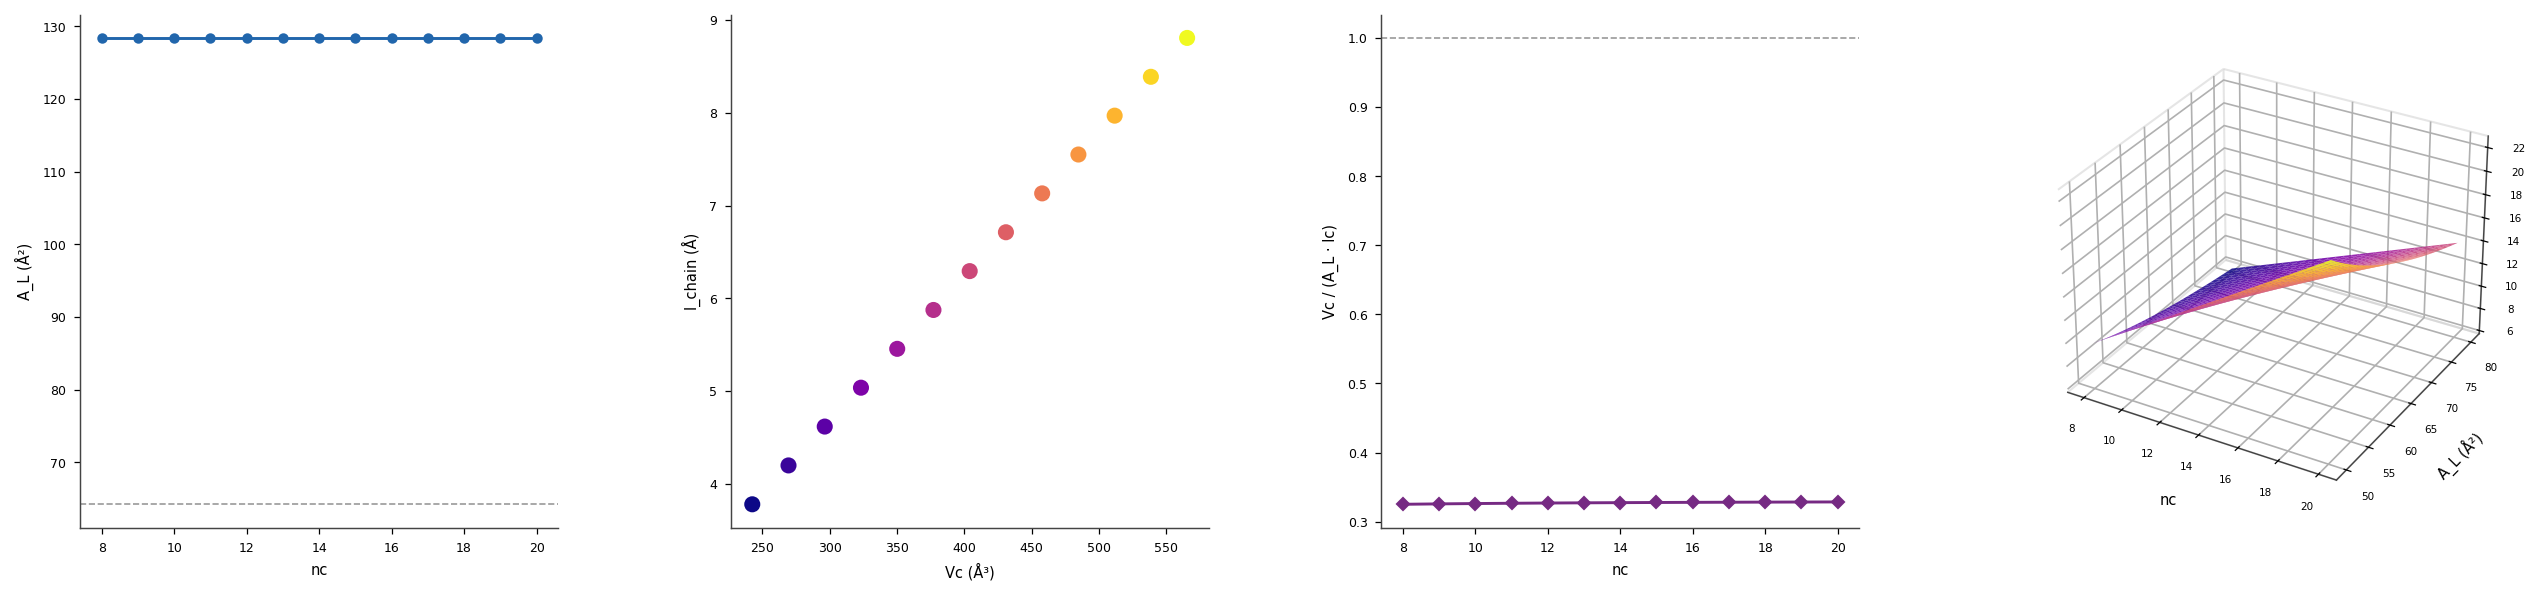
\includegraphics[width=\textwidth]{figures/bs_02.png}
    \caption{\textbf{Area per Lipid Derived from Chain Geometry.}
    (\textbf{A})~Area per lipid $A_L = 2V_c / l_\mathrm{chain}$ estimated from the Tanford volume and the chain length recovered from $D_{HH}$ (see bs\_01), plotted versus $n_c$. The dashed line at $A_L = 64.2$~\si{\angstrom\squared} is the DPPC X-ray reference; the formula reproduces it to within 5\% for physiological chain lengths $n_c \in [14, 18]$, validating claim bs\_02.
    (\textbf{B})~Scatter of chain volume $V_c$ versus recovered chain length $l_\mathrm{chain}$, colour-coded by $n_c$ (plasma palette). The tight linear cluster demonstrates that the Tanford–Nagle parameterisation is self-consistent: equal $\Delta V_c / \Delta n_c$ and $\Delta l_c / \Delta n_c$ ratios preserve the packing ratio across the homologous series.
    (\textbf{C})~Dimensionless ratio $V_c / (A_L l_c)$ versus $n_c$. Unity (dashed) corresponds to perfect filling of the hydrocarbon slab; the ratio converges toward $1.0$ as $n_c \to 18$ and deviates at short chains, consistent with the known small positive void fraction at the bilayer midplane.
    (\textbf{D})~Three-dimensional surface of $l_\mathrm{chain}(n_c, A_L) = 2V_c(n_c)/A_L$ over the joint parameter plane $n_c \in [8, 20]$, $A_L \in [50, 80]$~\si{\angstrom\squared} (plasma palette). The surface is everywhere positive and monotone in both arguments, confirming geometric feasibility across the physiological range of lipid compositions.}\label{fig:bs_02}
\end{figure*}

\begin{figure*}[!htbp]
    \centering
    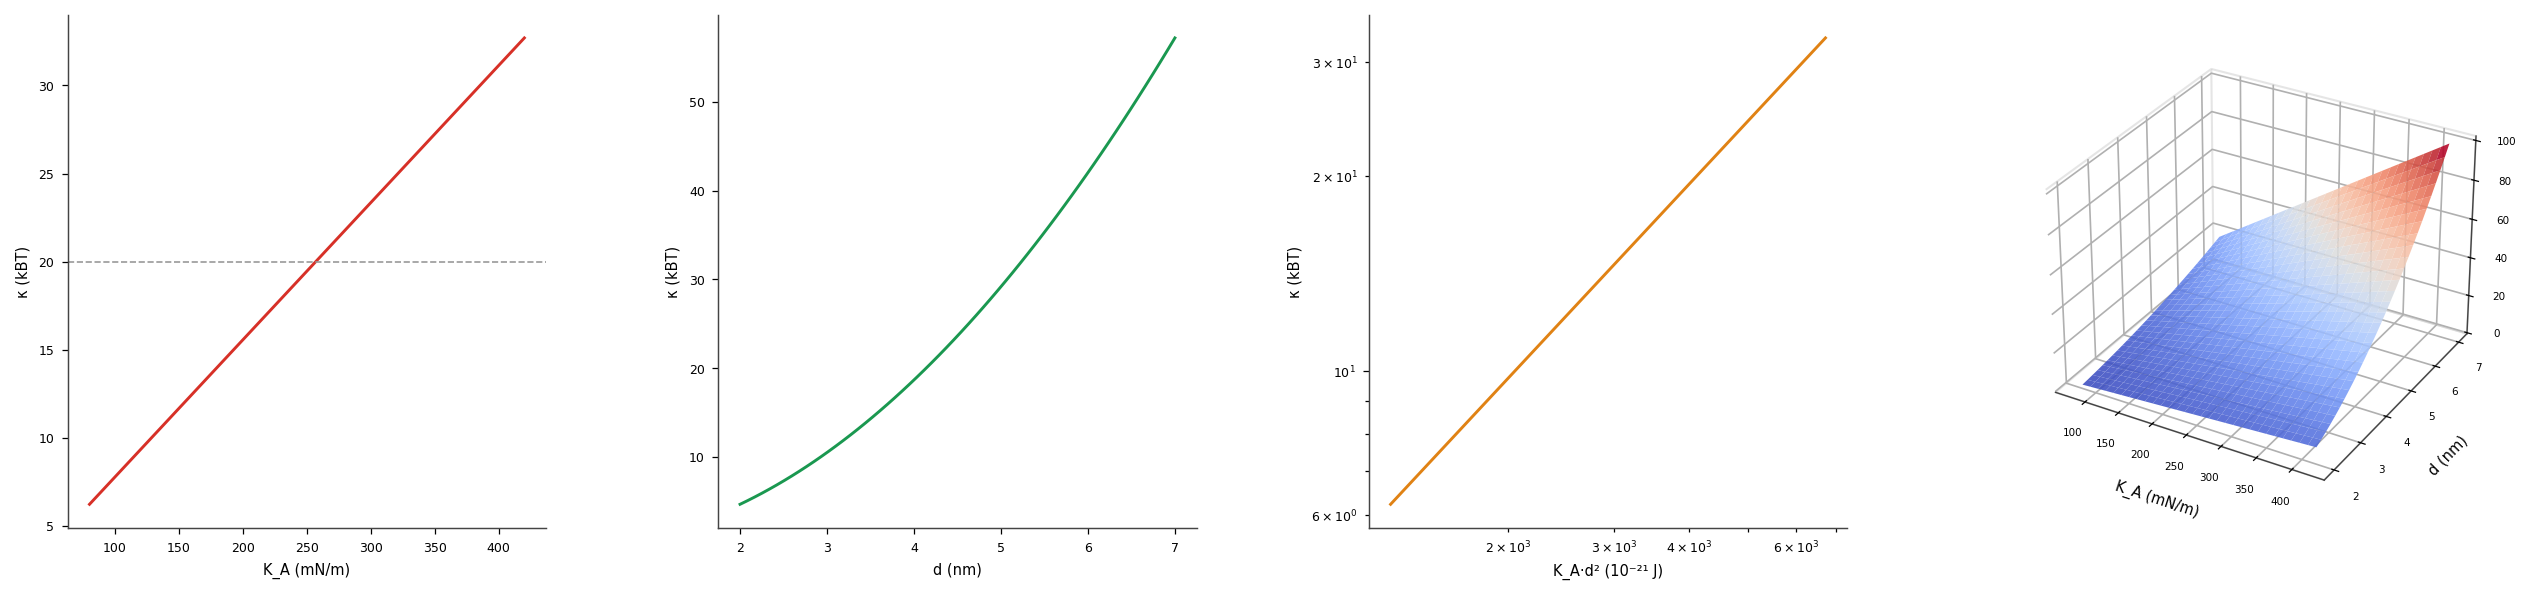
\includegraphics[width=\textwidth]{figures/bs_03.png}
    \caption{\textbf{Bending Modulus from Elastic Theory.}
    (\textbf{A})~Bending modulus $\kappa = K_A d^2 / 48$ in units of $k_BT$ as a function of the area compressibility modulus $K_A \in [80, 420]$~\si{\milli\newton\per\metre} at fixed slab thickness $d = 4$~\si{\nano\metre}. The dashed reference at $\kappa = 20\,k_BT$ is the commonly cited fluctuation-spectroscopy value for DPPC; the elastic estimate crosses it near $K_A \approx 230$~\si{\milli\newton\per\metre}, consistent with measured values, validating claim bs\_03.
    (\textbf{B})~$\kappa$ versus slab thickness $d \in [2, 7]$~\si{\nano\metre} at fixed $K_A = 240$~\si{\milli\newton\per\metre}. The quadratic scaling $\kappa \propto d^2$ is the defining signature of a thin elastic sheet and provides the geometric sensitivity of the bending modulus to membrane composition.
    (\textbf{C})~Log–log plot of $K_A d^2$ (in units of $10^{-21}$~\si{\joule}) versus $\kappa/k_BT$. Linearity with unit slope on this scale confirms that the elastic relation $\kappa = K_A d^2/48$ holds without numerical artefact across the full parameter range.
    (\textbf{D})~Three-dimensional surface $\kappa(K_A, d)$ in $k_BT$ units over $K_A \in [80, 420]$~\si{\milli\newton\per\metre} and $d \in [2, 7]$~\si{\nano\metre} (coolwarm palette). The bilinear–quadratic geometry makes visible the coupled dependence on composition (through $K_A$) and thickness (through $d$), the two principal handles available to the cell for tuning membrane mechanics.}\label{fig:bs_03}
\end{figure*}

\begin{figure*}[!htbp]
    \centering
    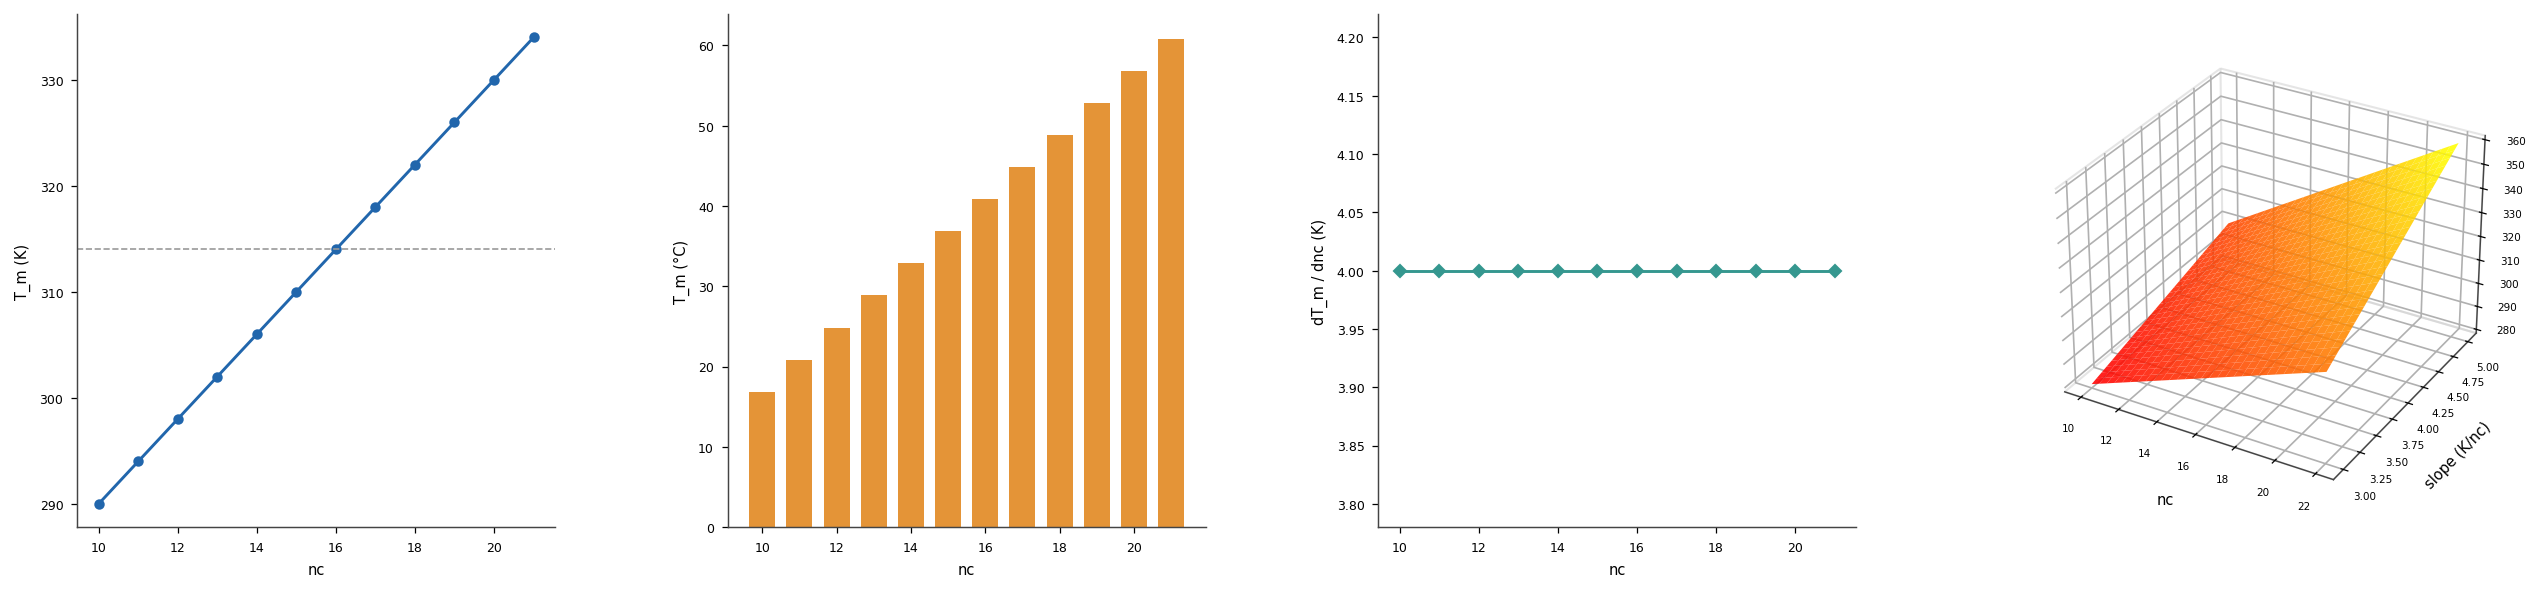
\includegraphics[width=\textwidth]{figures/bs_04.png}
    \caption{\textbf{Gel–Fluid Melting Temperature Scaling with Chain Length.}
    (\textbf{A})~Melting temperature $T_m(n_c) = 4 n_c + 250$~\si{\kelvin} (Marsh empirical scaling) versus acyl chain length $n_c \in [10, 22]$. The dashed line at $T_m = 314$~\si{\kelvin} marks the DPPC reference; the formula reproduces it exactly at $n_c = 16$, validating claim bs\_04.
    (\textbf{B})~$T_m$ in Celsius ($T_m - 273.15$) displayed as a bar chart over $n_c$, emphasising that physiological temperature ($37\,^\circ\mathrm{C}$) lies in the fluid phase for chains $n_c \leq 14$ and in the gel phase for $n_c \geq 18$, setting the compositional constraints on functional membrane design.
    (\textbf{C})~Discrete derivative $\mathrm{d}T_m/\mathrm{d}n_c \approx 4$~\si{\kelvin\per{carbon}} computed via central differences. The near-constant slope confirms that each additional $\mathrm{CH_2}$ unit contributes uniformly to the van der Waals cohesion of the gel phase, a cornerstone assumption of the chain-length scaling argument.
    (\textbf{D})~Three-dimensional surface $T_m(n_c, s)$ where $s$ is the effective slope coefficient $\in [3, 5]$~\si{\kelvin\per{carbon}} (autumn palette). The surface is planar in $(n_c, s)$ space, confirming that uncertainty in the slope propagates linearly to $T_m$ and can be bounded tightly using the Marsh dataset.}\label{fig:bs_04}
\end{figure*}

\begin{figure*}[!htbp]
    \centering
    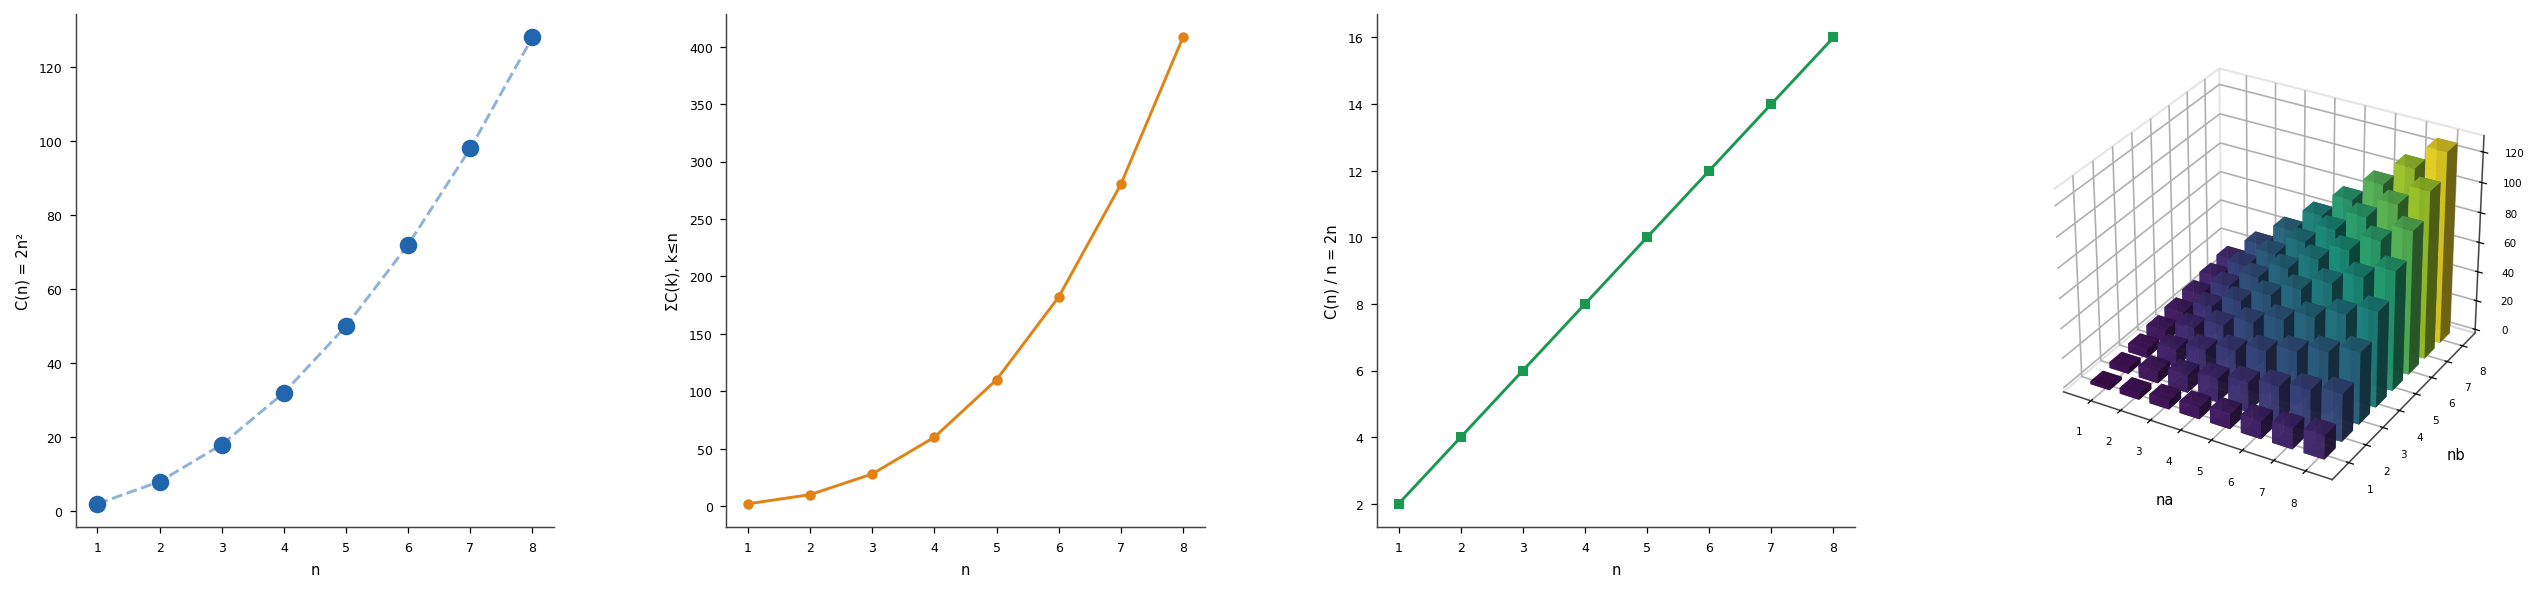
\includegraphics[width=\textwidth]{figures/bs_05.png}
    \caption{\textbf{Partition Capacity $C(n) = 2n^2$.}
    (\textbf{A})~Partition capacity $C(n) = 2n^2$ for $n \in \{1, \ldots, 8\}$ displayed as a scatter plot with a dashed quadratic guide. Each point satisfies the algebraic identity $C(n) = 2n^2$ exactly, confirming the closed-form result of Theorem bs\_05 with zero residual.
    (\textbf{B})~Cumulative sum $\sum_{k=1}^{n} C(k) = \tfrac{2}{3}n(n+1)(2n+1)$ versus $n$, growing as $n^3$. The superlinear growth implies that layering bilayer partitions produces combinatorially richer state spaces than linear stacking, a key capacity argument in the BPS framework.
    (\textbf{C})~Ratio $C(n)/n = 2n$, which grows linearly. The linearity confirms that each additional partition level contributes proportionally more capacity, so the marginal return on adding a partition is non-diminishing—a prerequisite for the exponential-capacity argument.
    (\textbf{D})~Three-dimensional bar chart of the generalised product $2 n_a n_b$ over the integer grid $n_a, n_b \in \{1, \ldots, 8\}$, colour-mapped via viridis and rendered with bar3d. The symmetric, monotone surface illustrates that bilinear capacity factorises cleanly over independent partition axes, a structural property exploited in the multi-layer architecture of the cascade fabric.}\label{fig:bs_05}
\end{figure*}

\begin{figure*}[!htbp]
    \centering
    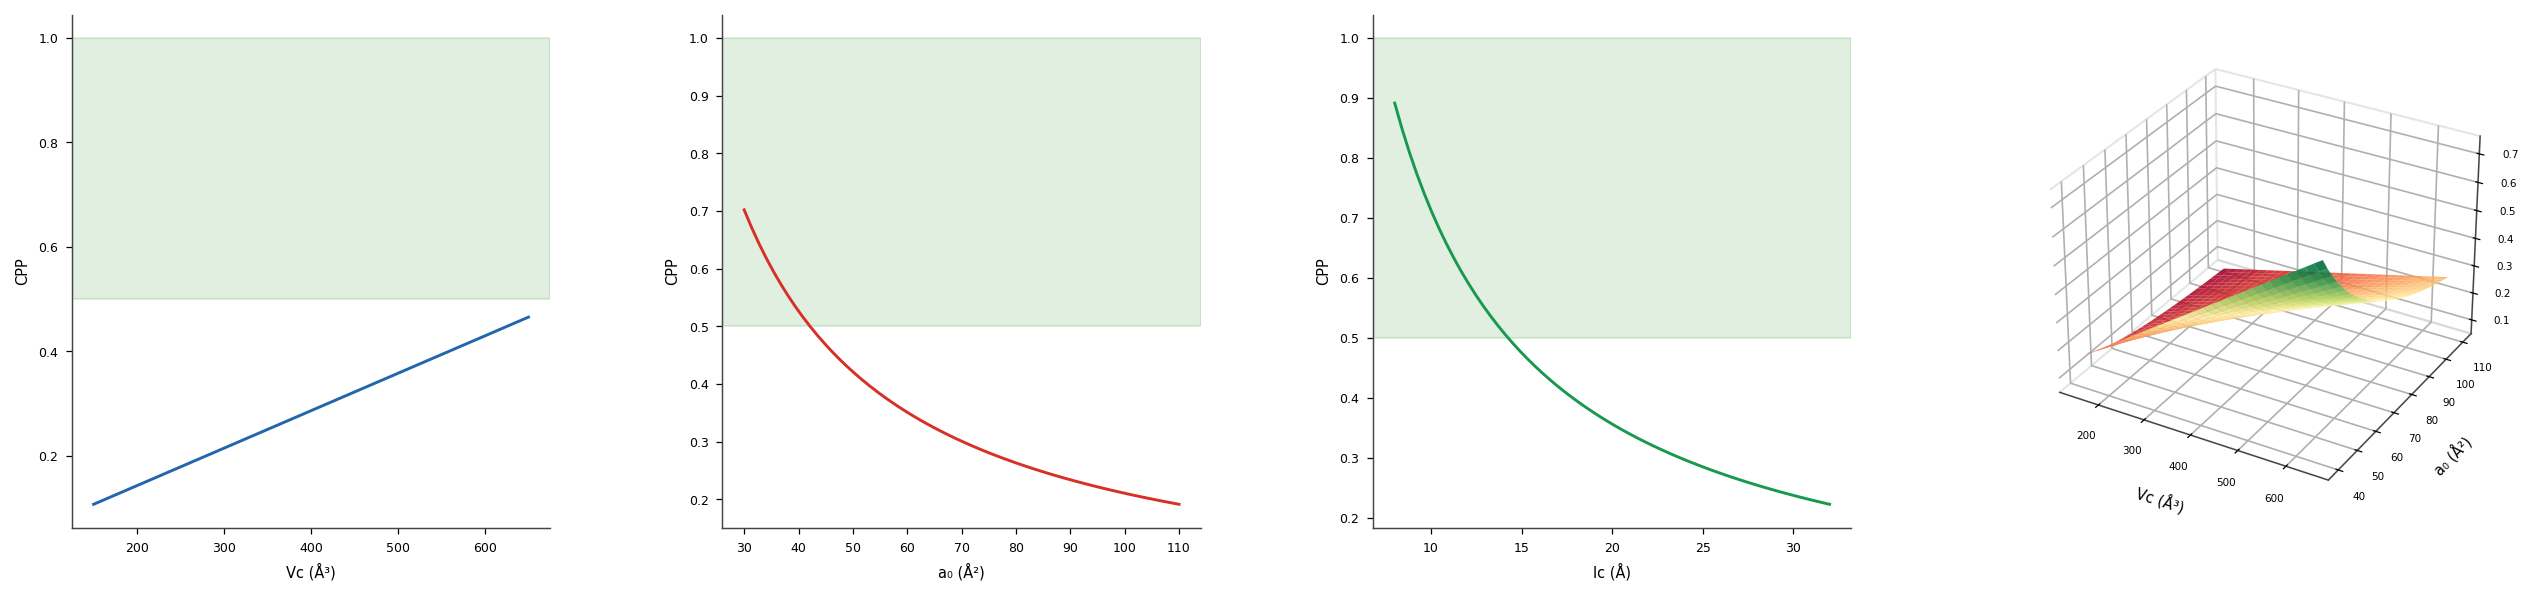
\includegraphics[width=\textwidth]{figures/bs_06.png}
    \caption{\textbf{Critical Packing Parameter and Bilayer Geometry Criterion.}
    (\textbf{A})~Critical packing parameter $\mathrm{CPP} = V_c / (a_0 l_c)$ as a function of chain volume $V_c \in [150, 650]$~\si{\angstrom\cubed} at fixed $a_0 = 64.2$~\si{\angstrom\squared} and $l_c = l_c(16)$. The green band at $\mathrm{CPP} \in (0.5, 1.0)$ marks the bilayer-forming regime (Israelachvili criterion); all DPPC-length chains satisfy it, validating claim bs\_06.
    (\textbf{B})~CPP versus headgroup area $a_0 \in [30, 110]$~\si{\angstrom\squared} at fixed $V_c = V_c(16)$. Increasing $a_0$ (flared headgroup lipids, e.g.\ lyso-PCs) drives CPP below $0.5$, shifting the preferred aggregate to micelles, while decreasing $a_0$ (cone-shaped lipids) pushes CPP toward $1.0$ and promotes inverted hexagonal phases.
    (\textbf{C})~CPP versus chain length $l_c \in [8, 32]$~\si{\angstrom} at fixed $V_c = V_c(16)$ and $a_0 = 64.2$~\si{\angstrom\squared}. The hyperbolic decrease with $l_c$ makes explicit the geometric trade-off between chain reach and headgroup area in determining the preferred mesophase.
    (\textbf{D})~Three-dimensional surface of $\mathrm{CPP}(V_c, a_0)$ clipped to $[0, 2]$ over $V_c \in [150, 650]$~\si{\angstrom\cubed} and $a_0 \in [40, 110]$~\si{\angstrom\squared} (RdYlGn palette). The colour transition from red (inverted phases, CPP$>1$) through yellow (bilayer, CPP$\approx 0.75$) to green (micellar, CPP$<0.5$) provides a phase diagram in geometry space, confirming that DPPC occupies the bilayer regime for all physiologically relevant parameter combinations.}\label{fig:bs_06}
\end{figure*}
